\section{Zellul\"arer Automat}
\label{sec:cellular_automaton}

%Damit die mobilen Geräten den Nutzern Hinweise zum nächsten Notausgang geben können, müssen sie ihre eigene Position kennen. Daher soll ein dezentraler Lokalisierungsalgorithmus implementiert werden (siehe [2]). Beispielweise kann der minimale Nachrichten Hop-Count zu einem Notausgang im Zusammenhang mit der maximalen Kommunikationsreichweite zur Ap-proximation der Distanz des Knotens zum Ausgang dienen (siehe [1], gradient algorithm). Meh-rere (>=3) dieser Distanzen können wiederum zur Positionierung verwendet werden (Stichwort: Lateration. Siehe multilateration algorithm in [1] oder Bogenschnitt). In der Visualisierung sollte die Qualität der Positionierung erkennbar sein, d.h. es sollte zusätzlich zur wahren Position des Sensorknotens die errechnete Position erkennbar sein

Die mobilen Geräte bestimmen über die \emph{Multilateration Lokalisierung} die approximierte Position der Personen. Daraus wird die Entfernung zu den Notausgängen geschätzt. Im Falle einer Gefahrensituation flüchten die Personen zu dem nächst gelegenen und verfügbaren Notausgang.

Für die Orientierung während der Flucht steuert die Umgebung (Zelluläre Automaten) die Bewegung der Person.

Die zellulären Automaten dienen zur Modellierung räumlich diskreter dynamischer Systeme. In diesem Fall wird die zweidimensionale Simulationsumgebung als Zellularraum $Z$ und die Patches als Zellen $z \in Z$ betrachtet. Die Patches bilden ein orthogonales Gitter.

Für die endliche Nachbarschaft der Zellen ergibt sich:

\begin{quote}
$ N_{Moore}(z)=\left\{\begin{array}{cl} \vert Z_{Neighbor}\vert = 3, & \mbox{falls }Edge(z) = true,\\ \vert Z_{Neighbor}\vert = 5, & \mbox{falls }Border(z) = true,\\ \vert Z_{Neighbor}\vert = 8, & \mbox{sonst.} \end{array}\right. $

$ N_{Neumann}(z)=\left\{\begin{array}{cl} \vert Z_{Neighbor}\vert = 2, & \mbox{falls }Edge(z) = true,\\ \vert Z_{Neighbor}\vert = 3, & \mbox{falls }Border(z) = true,\\ \vert Z_{Neighbor}\vert = 4, & \mbox{sonst.} \end{array}\right. $
\end{quote}

Abbildung \ref{fig:neighborhood} visualisiert die beiden Nachbarschaftsbeziehungen, Moore-Nachbarschaft $ N_{Moore}(z)$ oder Von-Neumann-Nachbarschaft $ N_{Neumann}(z)$, für die drei Zelltypen. Zelle $z_{1}$ ist an der oberen Ecke des Raumes, Zelle $z_{2}$ am Rand und Zelle $z_{3}$ innerhalb des Zellularraums. 

\begin{figure}[!ht]
\centering
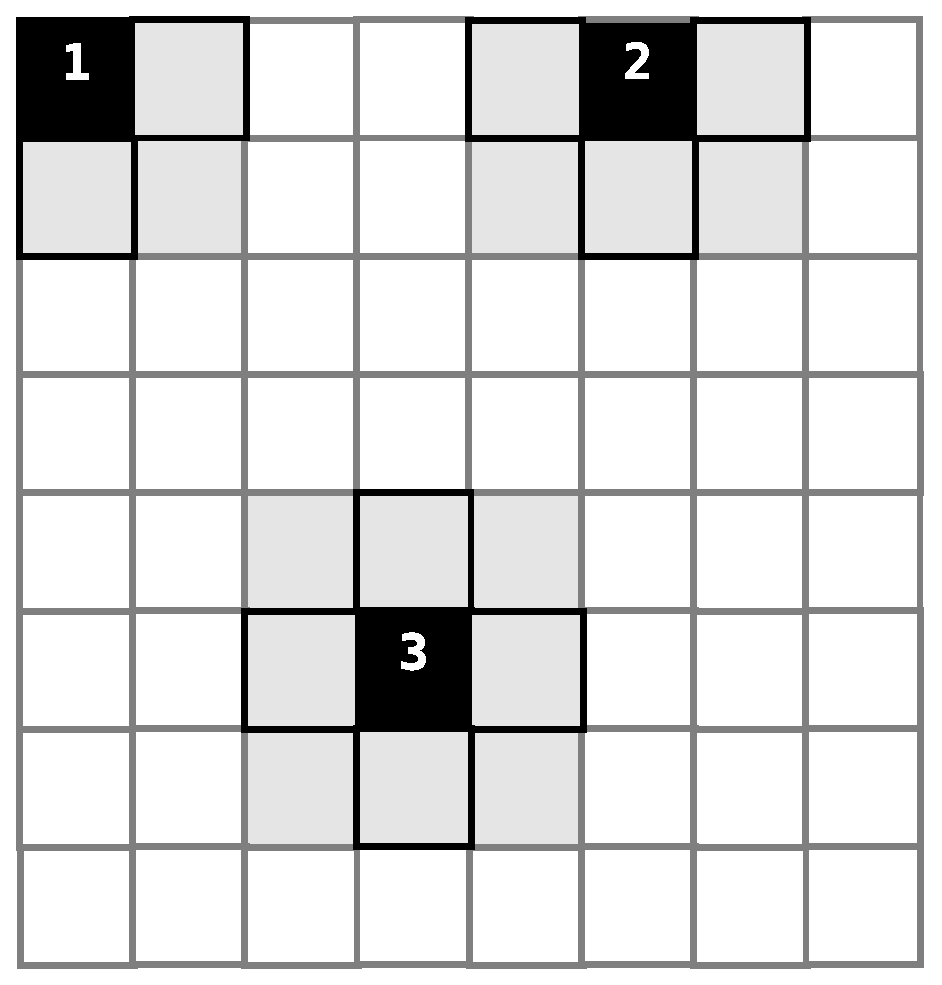
\includegraphics[height=0.3\textwidth]{algorithmik/neighborhood.eps}
\caption{Nachbarschaftsbeziehungen der Zellen}
\label{fig:neighborhood}
\end{figure}

Neben der Menge an benachbarten Zellen besitzt jede Zelle einen diskreten Zustand $q \in Q$ aus der Zustandsmenge $Q$, die bereits in Abschnitt \ref{sec:patch_states} angesprochen wurde.

\begin{quote}
$Q = \{NONE, SPREADING, IDLE, DONE\}$
\end{quote}

Zusätzlich besitzt jede Zelle lokale Zustandsübergangsregeln $\delta \colon Q^{N}\to Q$, die in Abhängigkeit mit den Zuständen und Werte aller Nachbarn zum Zeitpunkt $t$ deren neuen Zustand bestimmt. Für jeden diskreten Zeitschritt $t + 1$ werden die Zustandsübergangsregeln für alle Zellen angewendet.

Besonders ist hier, dass sowohl der Zustand einer Zelle überführt wird, als auch die Signalausbreitung der Notausgänge simuliert wird. Jede benachbarte Zelle $Z_{Neighbor} \subset Z\setminus\{z\}$ erhält den inkrementierten Signal-Dämpfungswert des Vorgängers $z \in Z$. Nachdem die dynamische Signalausbreitung abgeschlossen ist, werden die zellulären Automaten als terminiert, d.h. statisch angesehen. Zustands- und Wertänderungen sind nicht mehr möglich. Die Signalausbreitung ist beendet, sobald die maximale Dämpfung erreicht wurde.

Abbildung \ref{fig:flooding} zeigt die Zeitschritte $t_{1}$ bis $t_{9}$ bei Anwendung der Von-Neumann-Nachbarschaftsbeziehung. Die schwarze Zelle markiert die Position eines Notausgangs. Zum Zeitpunkt $t_{0}$ ist wird diese Zelle mit dem Signal-Dämpfungswert = 0 und dem Zustand \verb|SPREADING| (spontan) initialisiert.

\begin{figure}[!ht]
\centering
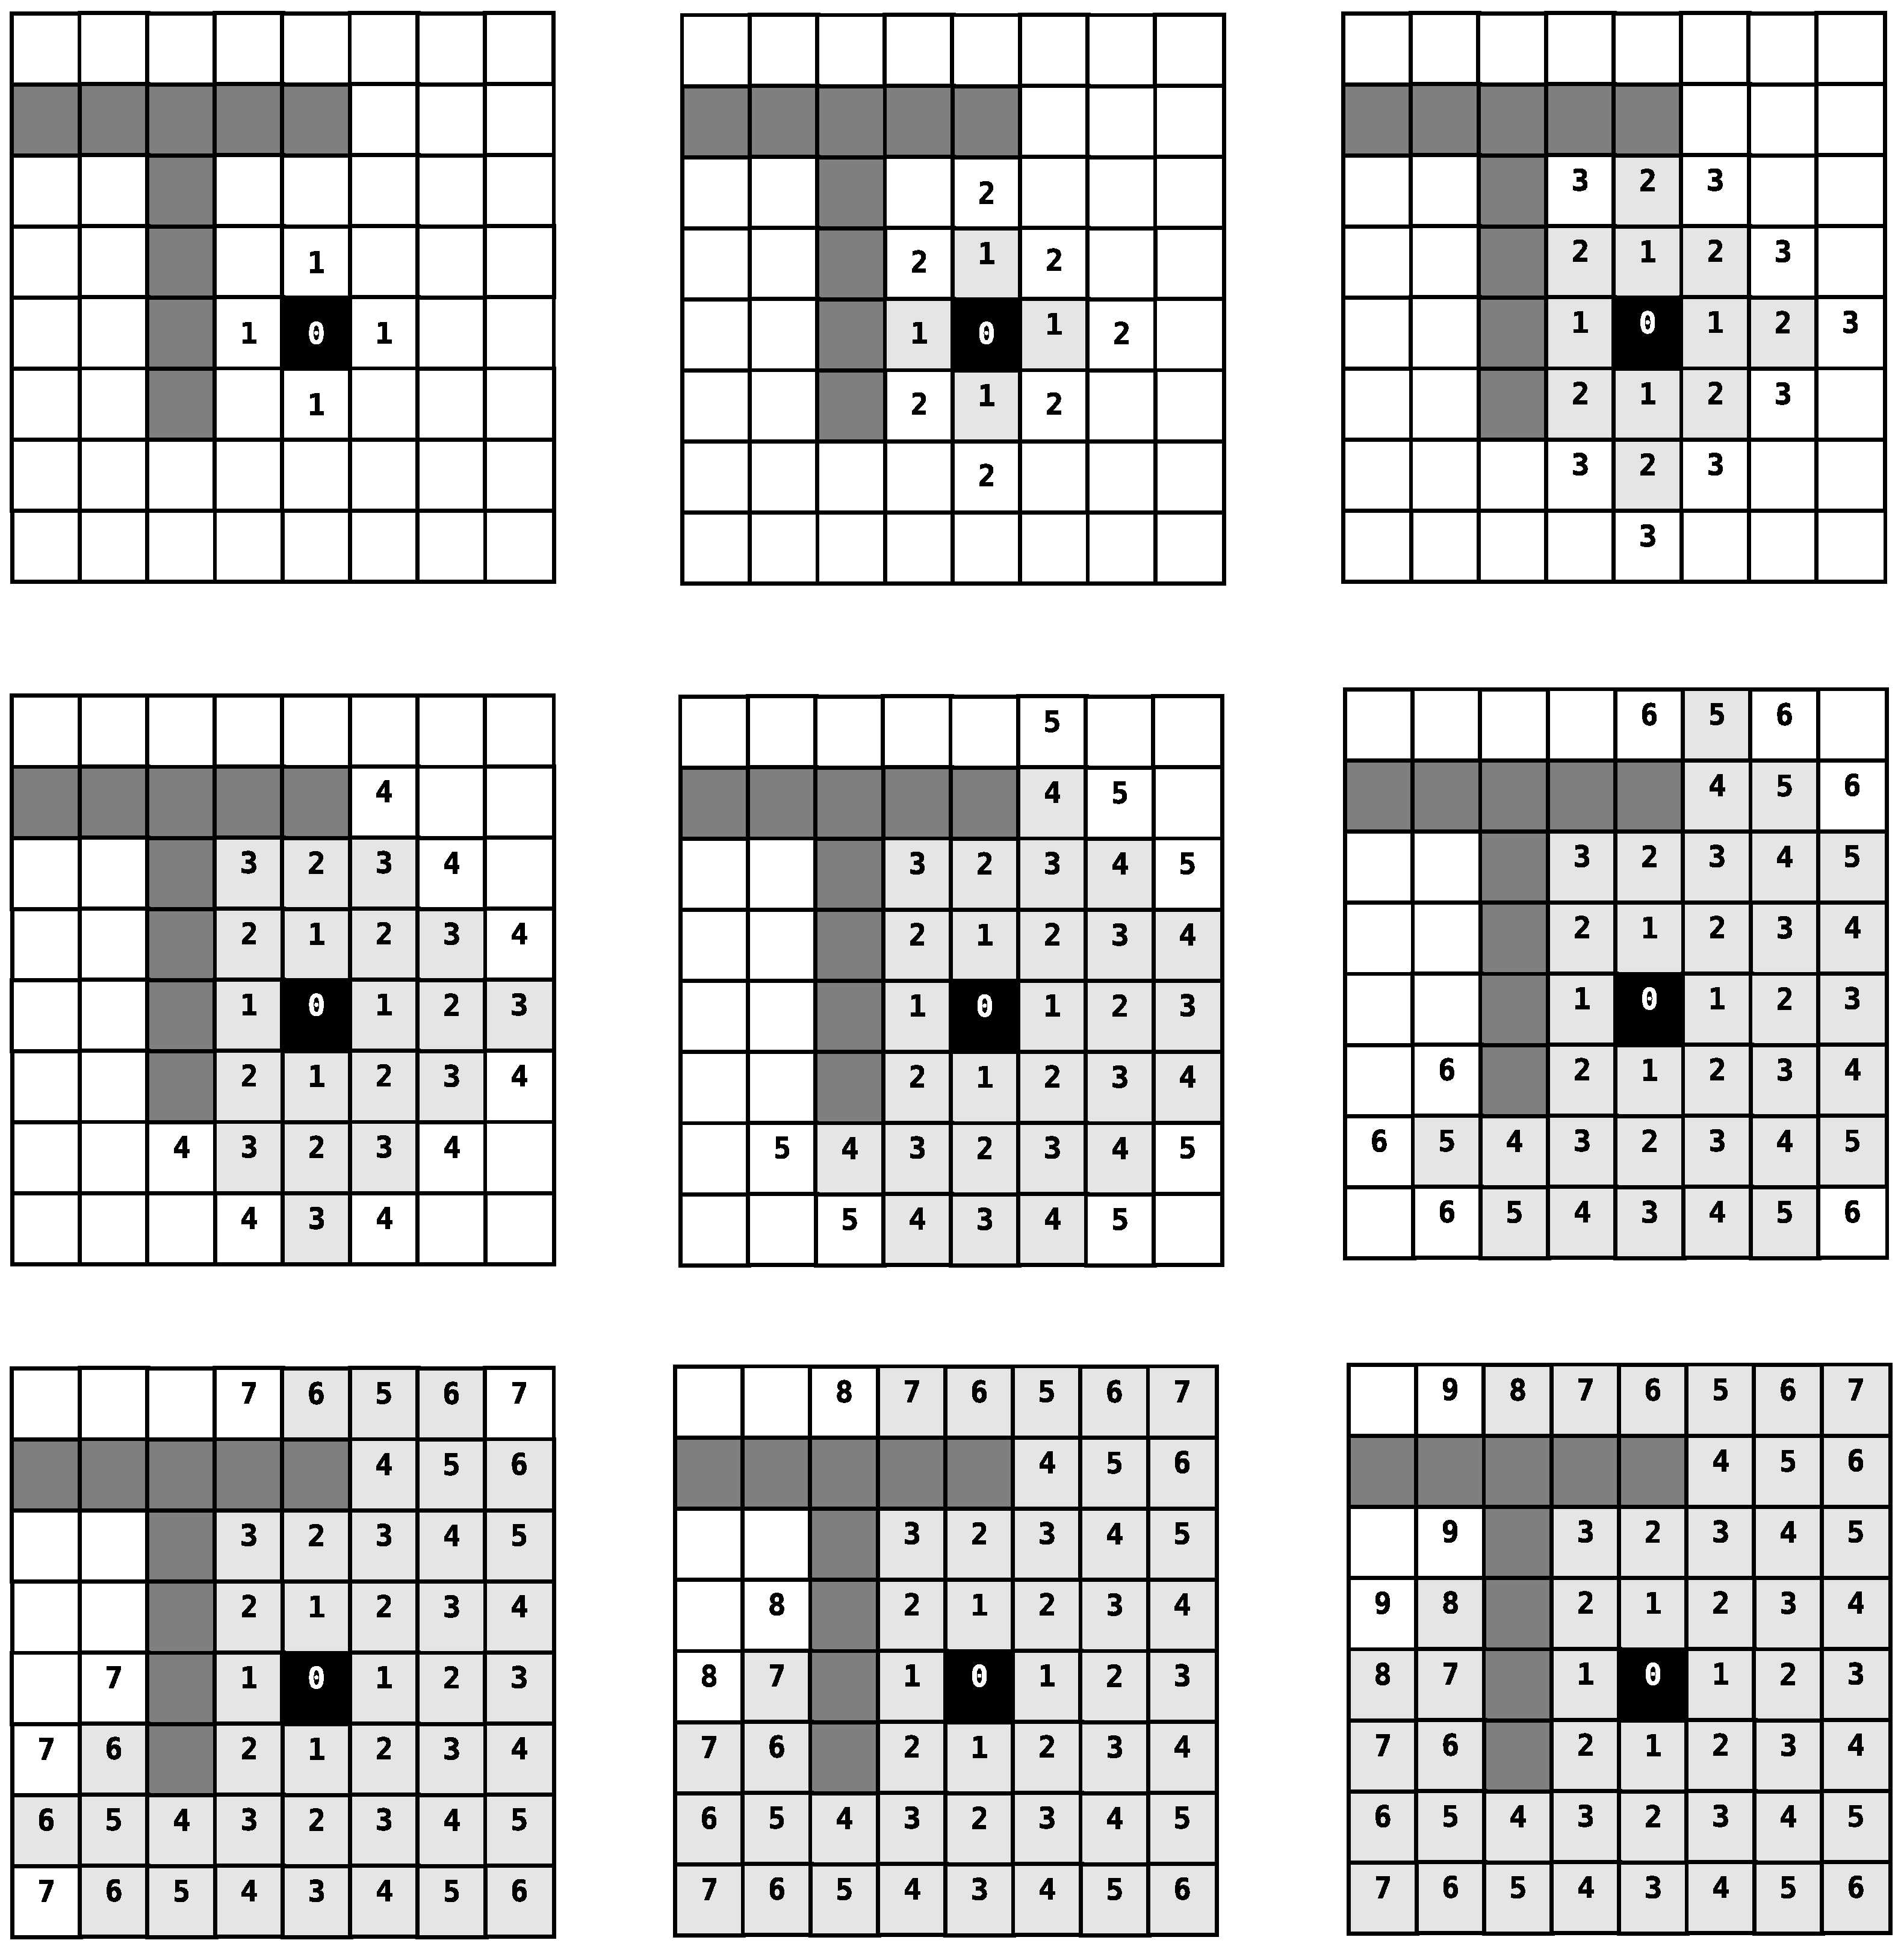
\includegraphics[height=0.9\textwidth]{algorithmik/flooding.eps}
\caption{Signalausbreitung eines Notausganges (Zelluläre Automaten)}
\label{fig:flooding}
\end{figure}

Die Signalausbreitung unterliegt dem lokalen Verhalten der zellulären Automaten durch die entsprechenden Zustandsübergangsregeln. Bei $i \geq 3$ Notausgängen sind die Zustandsübergangsregeln entsprechend komplex\footnote{Nach der Klassifizierung durch \cite{Wolfram} können die zellulären Automaten der Klasse 4 zugeordnet werden.} und werden an dieser Stelle nicht detailliert beschrieben.

\subsection{Orientierung der Personen bei der Flucht}

Nachdem die Signalausbreitung abgeschlossen ist, orientiert sich eine Person bei der Flucht anhand der lokalen Signal-Dämpfungswerten der aktuellen Zelle und der benachbarten Zellen. Das Bewegungsmodell wurde bereits in Abschnitt \ref{sec:bewegungsmodell} angeschnitten. Abbildung \ref{fig:fleeing} dient daher als visuelle Unterstützung der Fluchtwegbestimmung.

Zum Zeitpunkt $t_{-1}$ detektiert die Person eine Gefahrensituation. Die Person hat, über die \emph{Multilateration Lokalisierung} und der Kommunikation der Notausgänge, den Notausgang auf  $z_{exit} \in Z$ als nächstes verfügbares Evakuierungsziel bestimmt.

Die Person sei bei $t_{0}$ auf Zelle $z_{0} \in Z$ positioniert. Die Nachbarschaft sei mit $N_{Moore}(z_{0}) = Z_{z_{0}}$ gegeben. Anders als bei der Signalausbreitung bestimmt die Person den Fluchtweg über die Moore-Nachbarschaft. Der Vorteil liegt in der Möglichkeit diagonale Bewegungen auszuführen.

Die Ziel-Zelle $z_{i} \in Z$ für den nächsten Zeitschritt $t_{i}$  bestimmt die Person mittels der Funktion $N_{i}(Z_{z_{i-1}})$. Die Funktion $SN(z)$ liefert den Signal-Dämpfungswert einer Zelle.

\begin{quote}
$N_{i}(Z_{z_{i-1}}) \mathrel{\mathop:}= min(SN(z_{0_{u}})) = z_{i},$   $u = 1,...,\mid Z_{z_{i}}\mid$
\end{quote}

Entsprechend der Abbildung \ref{fig:fleeing} bestimmt die Person $t_{1}$, $t_{2}$ und $t_{3}$ folgende Ziel-Zellen:

\begin{quote}
($t_{1}$) $z_{1} = N_{1}(Z_{z_{0}}) = min(5,4,3,4, \infty , \infty , \infty , 6)$. $SN(z_{1}) = 3$\\

($t_{2}$) $z_{2} = N_{2}(Z_{z_{1}}) = min(\infty ,2,1,2,3,4,5,4)$. $SN(z_{2}) = 1$\\

($t_{3}$) $z_{3} = N_{3}(Z_{z_{2}}) = min(1,0,1,2,3,2,3,2)$. $SN(z_{3}) = 0$
\end{quote}

Erreicht eine Person eine Zelle mit dem Signal-Dämpfungswert $= 0$, versucht sie sich zu retten. Ist das Limit des Notausgangs bereits erreicht, sodass dieser blockiert, sucht sich die Person den nächstgelegenen verfügbaren Notausgang. Dafür ist eine Überlagerung der Signale von Notausgängen notwendig. Hinzu kommt die benötigte Verbindung zu einem verfügbaren Notausgang oder einer weiteren Person mit dem Wissen über einen verfügbaren Notausgang. Diese beiden Kriterien müssen erfüllt sein, sodass der Algorithmus zur Fluchtwegbestimmung funktioniert.

%Einteilung[Bearbeiten]
%
%Stephen Wolfram definiert in A New Kind of Science und in etlichen Arbeiten aus der Mitte der 1980er-Jahre vier Klassen, in die man die zellulären Automaten (genauer: die Regeln, die sie abarbeiten) je nach ihrem Verhalten unterteilen kann. Frühere Autoren versuchten lediglich, die Art der Muster für bestimmte Vorschriften zu ermitteln.
%Dem Aufwand nach geordnet waren dies die Klassen:
%Klasse 1: Fast alle ursprünglichen Muster entwickeln sich schnell zu einem stabilen und homogenen Zustand. Dadurch verschwindet jede Zufälligkeit in den ersten Mustern.
%Klasse 2: Fast alle ursprünglichen Muster entwickeln sich schnell in stabile oder oszillierende Strukturen. Einige Zufälligkeiten der ersten Muster kann man herausfiltern, jedoch können manche zurückbleiben. Lokale Änderungen am ursprünglichen Muster neigen dazu lokal zu bleiben.
%Klasse 3: Fast alle ursprünglichen Muster entwickeln sich pseudozufällig oder chaotisch. Jede stabile Struktur kann schnell durch Rauschen zerstört werden. Lokale Änderungen am ursprünglichen Muster neigen dazu, sich bis ins Unendliche auszubreiten.
%Klasse 4: Fast alle ursprünglichen Muster entwickeln sich in Strukturen, die vielschichtig und interessant interagieren. Endlich informative Ursprungsmuster können, wie in Klasse 2 üblich, stabile oder oszillierende Strukturen ergeben, aber die Anzahl der erforderlichen Schritte, um diesen Zustand zu erreichen, kann selbst für einfache Muster sehr groß sein. Lokale Änderungen am ursprünglichen Muster können sich bis ins Unendliche verbreiten.
%Wolfram hat vermutet, dass nicht alle zellulären Automaten der Klasse 4 dazu imstande sind, universelle Berechnungen auszuführen. Die Universalität hat sich vor allem für die Regel 110 und Conways Spiel des Lebens bestätigt.
%
%
%
%
%
%
%Die Von-Neumann-Nachbarschaft ist eine Nachbarschaftsbeziehung in einem quadratischen Raster. Lediglich die Flächen, welche eine Kante mit der Basisfläche gemeinsam haben, gelten als Nachbarn.
%Sie wurde nach John von Neumann benannt und wird auch als 4er-Nachbarschaft (bzw. Turmnachbarschaft aufgrund der Analogie zum Schach) bezeichnet.
%
%
%Die Moore-Nachbarschaft ist eine Nachbarschaftsbeziehung in einem quadratischen Raster. Alle Flächen, welche mindestens eine Ecke mit der Basisfläche gemeinsam haben, gelten als Nachbarn.
%Sie wurde nach Edward F. Moore benannt und wird auch als 8er-Nachbarschaft bezeichnet.




%Es gibt nur endlich viele Transitionsfunktionen f¨ur eine gegebene Zellenaufteilung.
%Bei n Nachbarn und k Farben gibt es nur kn+1 verschiedene Ausgangssituationen
%und k verschiedene Funktionswerte. Entsprechend ergeben sich daraus kkn+1
%verschiedene Transitionsfunktionen und damit zellul¨are Automaten.
%Entsprechend gibt es nur 223 = 256 verschiedene elementare zellul¨are Automaten.